%%%%%%%%%%%%%%%%%%%%%%%%%%%%%%%%%%%%%%%%%%%%%%%%%%%%%%%%%%%%%%%%%%%%%%
%%
%% RStemplate.tex
%%
%%   このテンプレートは,LaTeX-2e 専用です。
%%
%%
%%
%%%%%%%%%%%%%%%%%%%%%%%%%%%%%%%%%%%%%%%%%%%%%%%%%%%%%%%%%%%%%%%%%%%%%%
\documentclass[a4jsme]{jsmepaper}
\usepackage{rsympo}
\usepackage{jtygm}
\usepackage{bm}
\usepackage{epic,eepic}
\usepackage[dvipdfmx]{graphicx}

\pagestyle{empty}
%---------------------------------------------------------------------
% 和文主題
%---------------------------------------------------------------------
\title{
  ロボティクスシンポジア原稿体裁について
}
%---------------------------------------------------------------------
% 和文副題
%---------------------------------------------------------------------
\subtitle{
  --- 副題 ---
}
%---------------------------------------------------------------------
% 英文主題
%---------------------------------------------------------------------
\etitle{
  Paper Format for the Robotics Symposia
}
%---------------------------------------------------------------------
% 英文副題
%---------------------------------------------------------------------
\esubtitle{
  --- Sub-Title ---
}
%---------------------------------------------------------------------
% 著者和文名
%---------------------------------------------------------------------
\jauthor{
  炉簿 手楠$^{*1}$,\ \
  進歩 次亜$^{*2}$
}
%---------------------------------------------------------------------
% 著者英文名
%---------------------------------------------------------------------
\eauthor{
  Robo TEKUSU$^{*1}$ and
  Jia SINPO$^{*2}$
}
%---------------------------------------------------------------------
% 著者の所属の和文
%---------------------------------------------------------------------
\jaffiliation{
  $^{*1}$ & トキオ大学工学部ロボット工学科(〒111-1111 東京都大学区大学通り1-1-1)robo@robot.u-tokio.ac.jp\\
  $^{*2}$ & 古都大学大学院工学研究科進歩工学科(〒111-1111 京都市大学町744)sinpo@mech.koto-u.ac.jp
}
%---------------------------------------------------------------------
% 著者の所属の英文
%---------------------------------------------------------------------
\eaffiliation{
  $^{*1}$ Department of Robot Engineering, Tokio University \\
1-1-1 Daigaku-dori, Daigaku-ku, Tokyo 111-1111, Japan \\
  $^{*2}$Department of Shinpo Engineering, Koto University \\
744 Daigaku-chou, Kyoto 111-1111, Japan
}
%---------------------------------------------------------------------
% 英文の概要
%---------------------------------------------------------------------
\abstract{%
This template is written for the Robotics Symposia paper format
which is based on the macro package of J.S.M.E. paper form for \LaTeXe.
Please get the package from J.S.M.E home page to compile
the source file,
and refer the source file to prepare the manuscript for submitting.
%\abind
Abstract should be described by 100-200 words for summarizing the paper.
Xxxxxxxx xxxxxxxxxx xxx xxxxxxxxxxxxx xxxxxx xxxxxxxxxxx xxxxxxxxxxxx.
Xxxxxxxxxxxxxx xxx xxxxxxxxx x xxxxxxxxx xxxxxxxxxxxxxxxxxx xx xx xxxxxxx,
xxxxx xxxxxxx xxxxxxxx xxxxxxxxxx xx xxxxxxxxxxx xxxxxxxxxxx xxxxxxxxxx.
}
%---------------------------------------------------------------------
% キーワード
%---------------------------------------------------------------------
\keywords{Robotics Symposia, Paper format, \LaTeXe}
%---------------------------------------------------------------------
\begin{document}
\maketitle
\thispagestyle{empty}
%
\section{緒言}
本稿は,ロボティクスシンポジアの投稿論文の体裁についてまとめたものである.

論文は,A4用紙を用い,上下のマージンを25mm,左右のマージンを23mmとする.
原稿は6ページを基本とし,最大8ページまで認められる.
ただし,6ページを超過した場合,1ページあたり10,000円の超過料金が必要となる.

\section{題目,著者,所属,及びアブストラクト}
まず,論文の和文題目を「ゴシック体・14pts・ボールド・センタリング」で書く.
副題がある場合は,フォントサイズを12ptsとして``---"で挟む.
それ以外のフォーマットはタイトルに準拠する.
続いて和文著者氏名を「ゴシック・12pts・センタリング」で書く.
各著者氏名の後には,上付で注番号を付ける.
続けて
英文題目を「Times New Roman・12pts・ボールド・センタリング」で書く.
副題は同じ書式で書き,``---"で挟む.
その下に,
英文著者氏名を「Times New Roman・12pts・センタリング」で書き,
英文著者氏名の後にも,和文著者氏名の注番号に対応するように,上付で注番号を付ける.
英文著者氏名の下に英文所属を「Times New Roman・10pts・センタリング」で書く.
各英文所属の前には,著者氏名に対応する注番号を上付で付ける.
なお,和文の所属,住所,およびE-mailアドレスは脚注(1ページ目左下)にまとめる.
脚注の和文所属の前にも,著者氏名に対応する注番号を上付で付ける.

続いて,
英文アブストラクトを「Times New Roman・10pts」,100$\sim$200語,
その下に「Times New Roman・10pts」でキーワードを3$\sim$5語記述する.
本文はその下から書きはじめる.

\section{本文}
本文のレイアウトは2段組とし,1段当たり46行,1行24文字を基準とする.
使用する文字は「明朝体・10pts」を原則とし,
文章の区切りには全角の読点「,」と句点「.」を用いる.
半角かな文字を使用してはならない.

%-------------------------------------------------
%  Table 2 (tbl:units)
%-------------------------------------------------
\begin{table*}[htbp]
  \setcounter{table}{1}
  \begin{center}
  \caption{Examples of symbols and units}
  \label{tbl:units}
  \begin{tabular}{c||c|c|c|c|c|c|c|c}\hline
    Item   & Time    & Length  & Angular velocity & Acceleration & Mass  & Moment of inertia & Force & Torque   \\\hline
    Symbol & $t$     & $l$     & $\omega$         & $\alpha$     & $m$   & $I$               & $f$   & $\tau$   \\\hline
    Unit   & s       & m       & rad/s            & m/s$^2$      & kg    & kgm$^2$           & N     & Nm       \\\hline
    1      & x.xxxx  & x.xxx   & x.xxx            & x.xxx        & x.xxx & x.xxx             & x.xxx & x.xxx    \\\hline
    2      & x.xxxx  & x.xxx   & x.xxx            & x.xxx        & x.xxx & x.xxx             & x.xxx & x.xxx    \\\hline
    3      & 8.1409  & 1.285   & 4.301            & 0.023        & 3.112 & 2.207             & 0.444 & 6.008    \\\hline
    4      & x.xxxx  & x.xxx   & x.xxx            & x.xxx        & x.xxx & x.xxx             & x.xxx & x.xxx    \\\hline
  \end{tabular}
  \end{center}
\end{table*}
%-------------------------------------------------

\section{記号・単位}
数字,数学記号,量記号及び単位記号は半角英数字を使用し,
数学記号,及び量記号はイタリック体,単位記号はローマン体で書く.
単位は,SI単位を使用する.
量記号に単位を付ける場合は,$m$[kg] のように単位を半角大括弧でくくる.
また,数字に単位を付ける場合は 5kg のように括弧は付けない.

\section{見出し}
\subsection{章見出し}
章見出しは2行分を取り,行の中ほどに「ゴシック体・10pts・ボールド」で書く.
%(メニューの「書式」「段落」における「インデントと行間隔」のタブで,
%「間隔」の段落前と段落後を5ptに設定する.)
ただし18字以上は3 行分を取る.

\subsection{節見出し}
節見出しは本文と同じ体裁で「ゴシック体・10pts・ボールド」で書く.
本文は改行せず,節見出しの直後に2文字空白を空け書きはじめる.

\section{図・写真,及び表}
\begin{itemize}
\item[(1)] 本文中では,図1,表1のように日本語で書く.写真は図として扱う.
\item[(2)] 番号・説明などは,図・写真についてはその下に,
           表についてはその上に書く(図\ref{fig:sample},表\ref{tbl:symb}参照).
\item[(3)] 本文と図・表の間は1行以上の空白を空ける.
\item[(4)] 図中・表中の説明,及び題目はすべて英語で書く(最初の文字は大文字とする).
\item[(5)] 図,及び表がl段(片側)に収まらない場合,表\ref{tbl:units}のように2段(両側)にまたがって書いてもよい.
\item[(6)] 図,及び表の横に空白ができても,その空白部には本文を記入してはならない.
\end{itemize}
%-----------------------------------------------------------
%  Figure 1 (fig:sample)
%-----------------------------------------------------------
\begin{figure}[htbp]
  \begin{center}
  \vspace{1zh}
    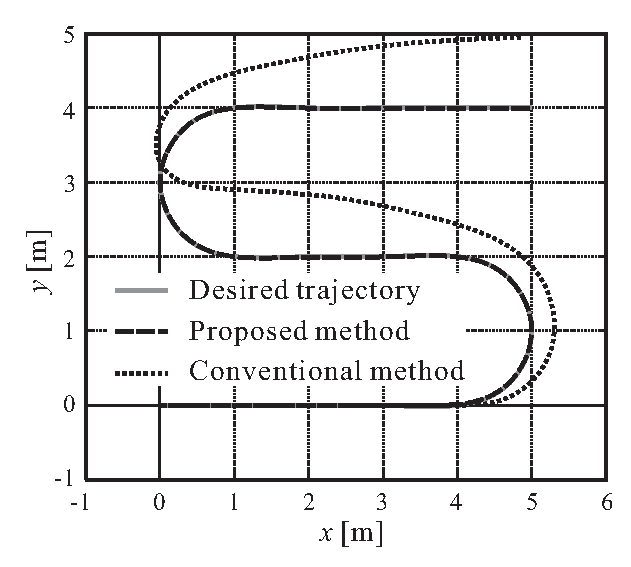
\includegraphics[width=65mm]{figs/fig.eps}
  \end{center}
  \caption{Sample figure}
  \label{fig:sample}
\end{figure}
%-----------------------------------------------------------

%-------------------------------------------------
% Table 1 (tbl:symb)
%-------------------------------------------------
\begin{table}[htbp]
  \setcounter{table}{0}
  \begin{center}
  \vspace{1zh}
  \caption{Sample expressions of values}
  \label{tbl:symb}
  \begin{tabular}{c|c}\hline
    Recommend     & Not recommend \\\dhline
    $\sqrt{x-y}$ & $\sqrt{ } (x-y)$ \\\hline
    $(a+b)/(c+d)$ & $a+b/c+d$        \\\hline
  \end{tabular}
  \end{center}
\end{table}
%-------------------------------------------------

\section{数式}
数式は次のようにセンタリングで書き,
式番号を式と同じ行に右寄せして小括弧の中に書く.
%-------------------------------------------------
% eq:dynamics1
%-------------------------------------------------
\begin{equation}
   \bm{\tau} = \bm{M}(\bm{q})\ddot{\bm{q}} + \bm{h}(\bm{q},\dot{\bm{q}}) + \bm{g}
\label{eq:dynamics1}
\end{equation}
%-------------------------------------------------
また,本文で式を引用するときは,式(\ref{eq:dynamics1})のように書く.
なお,本文と式,式相互間は1行以上の空白を空ける.
%また,原則として数式エディタのポイント数は本文に準じるものとするが,
%添え字等が小さく読みにくくなるときは適宜拡大する.

\section{参考文献}

参考文献については,本文中の引用箇所の右肩に,
小括弧付けで通し番号を付ける\cite{bibsample1,bibsample2,aaaa,bbbb}.
%例えば,新宿・渋谷(1)〜(3)のようにする.
文中で引用された参考文献は,
本文末尾に本文と対応する番号順でまとめて書く.
番号は引用と同様に小括弧でくくる.

\section{結言}
本サンプルファイルはすべての環境で動作,仕上がりを保証するものではありません.
ご使用の環境に合わせて,適宜,変更,微調整を行ってください.

%---------------------------------------------------------------------
% 参考文献
%---------------------------------------------------------------------
{\small
\begin{thebibliography}{99}
%
\bibitem{bibsample1}
    Robo TEKUSU,
    ``Xxxxxxxxxx xx Xxx Xxxxxx xxxx Xxxxxxxxx Xxxxxxxxx'',
    {\it Proceedings of the 2004 IEEE/RSJ International
    Conference on Intelligent Robot and Systems},
    (2004), pp.xxxx--xxxx.
%
\bibitem{bibsample2}
    Author First, Author Second and Author Third,
    ``XXXX XXXX Xxxxxxxxxx Xxxxxxxxx Xxxxxxxxx'',
    {\it IEEE Transactions on Robotics and Automation},
    Vol.17, No.3(1998), pp.xxx--xxx.
%
\bibitem{aaaa}
    進歩 次亜,
    “正しい投稿論文の書き方”,
    山口出版, (2002),
    pp.128--158.
%
\bibitem{bbbb}
    著者 A,著者 B,
    “一脚移動ロボットの動作計画と検証実験”,
    日本機械学会論文集C編,
    Vol.82,No.945 (2009), pp.xxx--xxx.
\end{thebibliography}}

\end{document}
